\documentclass{article}
\usepackage{amsfonts, amsthm, amsmath, amssymb, mathtools, ulem, mathrsfs, physics, esint, siunitx, tikz-cd}
\usepackage{pdfpages, fullpage, color, microtype, cancel, textcomp, markdown, hyperref, graphicx}
\usepackage{enumitem}
\usepackage{algorithm}
\usepackage{algpseudocode}
\graphicspath{{./images/}}
\usepackage[english]{babel}
\usepackage[autostyle, english=american]{csquotes}
\MakeOuterQuote{"}
\usepackage{xparse}
\usepackage{tikz}

\usepackage{calligra}
\DeclareMathAlphabet{\mathcalligra}{T1}{calligra}{m}{n}
\DeclareFontShape{T1}{calligra}{m}{n}{<->s*[2.2]callig15}{}
\newcommand{\script}[1]{\ensuremath{\mathcalligra{#1}}}
\newcommand{\scr}{\script r}

% fonts
\def\mbb#1{\mathbb{#1}}
\def\mfk#1{\mathfrak{#1}}
\def\mbf#1{\mathbf{#1}}
\def\tbf#1{\textbf{#1}}

% common bold letters
\def\bP{\mbb{P}}
\def\bC{\mbb{C}}
\def\bH{\mbb{H}}
\def\bI{\mbb{I}}
\def\bR{\mbb{R}}
\def\bQ{\mbb{Q}}
\def\bZ{\mbb{Z}}
\def\bN{\mbb{N}}

% brackets
\newcommand{\br}[1]{\left(#1\right)}
\newcommand{\sbr}[1]{\left[#1\right]}
\newcommand{\brc}[1]{\left\{#1\right\}}
\newcommand{\lbr}[1]{\left\langle#1\right\rangle}

% vectors
\renewcommand{\i}{\hat{\imath}}
\renewcommand{\j}{\hat{\jmath}}
\renewcommand{\k}{\hat{k}}
\newcommand{\proj}[2]{\text{proj}_{#2}\br{#1}}
\newcommand{\m}[2][b]{\begin{#1matrix}#2\end{#1matrix}}
\newcommand{\arr}[3][\sbr]{#1{\begin{array}{#2}#3\end{array}}}

% misc
\NewDocumentCommand{\seq}{O{n} O{1} O{\infty} m}{\br{#4}_{{#1}={#2}}^{#3}}
\NewDocumentCommand{\app}{O{x} O{\infty}}{\xrightarrow{#1\to#2}}
\newcommand{\sm}{\setminus}
\newcommand{\sse}{\subseteq}
\renewcommand{\ss}{\subset}
\newcommand{\vn}{\varnothing}
\newcommand{\lc}{\epsilon_{ijk}}
\newcommand{\ep}{\epsilon}
\newcommand{\vp}{\varphi}
\renewcommand{\th}{\theta}
\newcommand{\cjg}[1]{\overline{#1}}
\newcommand{\inv}{^{-1}}
\DeclareMathOperator{\im}{im}
\DeclareMathOperator{\id}{id}
\newcommand{\ans}{\tbf{Ans. }}
\newcommand{\pf}{\tbf{Pf. }}
\newcommand{\imp}{\implies}
\newcommand{\impleft}{\reflectbox{$\implies$}}
\newcommand{\ck}{\frac1{4\pi\ep_0}}
\newcommand{\ckb}{4\pi\ep_0}
\newcommand{\sto}{\longrightarrow}
\DeclareMathOperator{\cl}{cl}
\DeclareMathOperator{\intt}{int}
\DeclareMathOperator{\bd}{bd}
\DeclareMathOperator{\Span}{span}
\newcommand{\floor}[1]{\left\lfloor#1\right\rfloor}
\newcommand{\ceil}[1]{\left\lceil#1\right\rceil}
\newcommand{\fxn}[5]{#1:\begin{array}{rcl}#2&\longrightarrow & #3\\[-0.5mm]#4&\longmapsto &#5\end{array}}
\newcommand{\sep}[1][.5cm]{\vspace{#1}}
\DeclareMathOperator{\card}{card}
\renewcommand{\ip}[2]{\lbr{#1,#2}}
\renewcommand{\bar}{\overline}
\DeclareMathOperator{\cis}{cis}
\DeclareMathOperator{\Arg}{Arg}
\newcommand{\ptl}{\partial}
\newcommand{\om}{\omega}

% title
\title{Scientific Computing HW 5}
\author{Ryan Chen}
%\date{\today}
\setlength{\parindent}{0pt}


\begin{document}
	
\maketitle



\tbf{Problem 1.}

\begin{enumerate}
	
\item From $H(p,q)=T(p)+U(q)$,
$$\ptl_pH(p,q) = T'(p),
\quad \ptl_qH(p,q) = U'(q)$$
Plug into the Stoermer--Verlet method.
$$p_{n+1/2} = p_n - \frac12hU'(q_n)$$
$$q_{n+1} = q_n + \frac12h[T'(p_{n+1/2}) + T'(p_{n+1/2})]
= q_n + hT'\br{p_n - \frac12hU'(q_n)}$$
$$p_{n+1} = p_n - \frac12hU'(q_n) - \frac12hU'(q_{n+1})
= p_n - \frac12h\sbr{U'(q_n) + U'\br{q_n + hT'\br{p_n - \frac12hU'(q_n)}}}$$
The RHS quantities are independent of $p_{n+1},q_{n+1}$, so the method is explicit.\\

The Hamiltonian for the 1D simple harmonic oscillator is
$$H(p,q) = T(p) + U(q),
\quad T(p) := \frac{p^2}{2m},
\quad U(q) := \frac{m\om^2q^2}{2}$$
First compute
$$T'(p) = \frac pm,
\quad U'(q) = m\om^2q$$
Plug into the method.
$$q_{n+1} = q_n + hT'\br{p_n - \frac12hm\om^2q_n}
= q_n + \frac hm\sbr{p_n - \frac12h\om^2q_n}
= \frac hmp_n + \br{1 - \frac12h^2\om^2}q_n$$
$$p_{n+1} = p_n - \frac12h\sbr{m\om^2q_n + m\om^2\br{q_n + \frac hm\br{p_n - \frac12hm\om^2q_n}}}$$
In the above expression, collect coefficients of the following terms.
\begin{align*}
	p_n &: \quad 1 - \frac12hm\om^2\frac hm = 1 - \frac12h^2\om^2 \\
	q_n &: \quad -\frac12h\sbr{m\om^2 + m\om^2\br{1+ \frac hm\br{-\frac12hm\om^2}}}
	= -\frac12hm\om^2\br{2 - \frac12h^2\om^2}
	= hm\om^2\br{\frac14h^2\om^2 - 1}
\end{align*}
Therefore
$$\m{p_{n+1} \\ q_{n+1}} = A\m{p_n \\ q_n},
\quad A := \m{a & b \\ c & a},
\quad a := 1 - \frac12h^2\om^2,
\quad b := hm\om^2\br{\frac14h^2\om^2 - 1},
\quad c := \frac hm$$


\item \pf We compute
$$JA = \m{0 & 1 \\ -1 & 0}\m{a & b \\ c & a}
= \m{c & a \\ -a & -b}$$
$$\imp A^TJA = \m{a & c \\ b & a}\m{c & a \\ -a & -b}
= \m{ac-ca & a^2-bc \\ bc-a^2 & ba-ab}
= \m{0 & a^2-bc \\ -(a^2-bc) & 0}$$
$$a^2 - bc = 1 + \frac14h^4\om^4 - h^2\om^2 - h^2\om^2\br{\frac14h^2\om^2 - 1}
= 1 + \frac14h^4\om^4 - h^2\om^2 - \frac14h^4\om^4 + h^2\om^2
= 1$$
$$\imp A^TJA = \m{0 & 1 \\ -1 & 0} = J$$


\item \pf The shadow Hamiltonian is
$$H^*(p_n,q_n) = \frac{p_n^2}{2m} + \frac12m\om^2q_n^2\sbr{1 - \frac14h^2\om^2}
= \m{p_n \\ q_n}^T S \m{p_n \\ q_n},
\quad S := \m{d & 0 \\ 0 & e},
\quad d := \frac1{2m},
\quad e := \frac12m\om^2\sbr{1 - \frac14h^2\om^2}$$
We compute
$$SA = \m{d & 0 \\ 0 & e}\m{a & b \\ c & a}
= \m{da & db \\ ec & ea}$$
$$\imp A^TSA = \m{a & c \\ b & a}\m{da & db \\ ec & ea}
= \m{da^2+ec^2 & dba+eac \\ bda+aec & db^2+ea^2}
= \m{da^2+ec^2 & a(bd+ec) \\ a(bd+ec) & db^2+ea^2}$$
$$bd + ec = \frac12h\om^2\sbr{\frac14h^2\om^2 - 1} + \frac12h\om^2\sbr{1 - \frac14h^2\om^2} = 0$$
\begin{align*}
	da^2 + ec^2 &= \frac{1}{2m}\sbr{1 + \frac14h^4\om^4 - h^2\om^2} + \frac12m\om^2\sbr{1 - \frac14h^2\om^2}\frac{h^2}{m^2}\\
	&= \frac{1}{2m}\sbr{1 + \frac14h^4\om^4 - h^2\om^2 + h^2\om^2 - \frac14h^4\om^4}\\
	&= \frac{1}{2m}\\
	&= d\\		
	db^2 + ea^2 &= \frac{1}{2m}h^2m^2\om^4\sbr{\frac14h^2\om^2 - 1}^2 + \frac12m\om^2\sbr{1 - \frac14h^2\om^2}\sbr{1 + \frac14h^4\om^4 - h^2\om^2} \\
	&= \frac12m\om^2\sbr{1-\frac14h^2\om^2}\sbr{h^2\om^2\br{1 - \frac14h^2\om^2} + 1 + \frac14h^4\om^4 - h^2\om^2}\\
	&= \frac12m\om^2\sbr{1-\frac14h^2\om^2}\sbr{h^2\om^2 - \frac14h^4\om^4 + 1 + \frac14h^4\om^4 - h^2\om^2}\\
	&= \frac12m\om^2\sbr{1-\frac14h^2\om^2}\\
	&= e	
\end{align*}
Put together,
$$A^TSA = \m{d & a\cdot0 \\ a\cdot0 & e} = \m{d & 0 \\ 0 & e} = S$$
$$\imp H^*(p_{n+1},q_{n+1}) = \m{p_{n+1} \\ q_{n+1}}^TS\m{p_{n+1} \\ q_{n+1}}
= \m{p_{n} \\ q_{n}}^TA^TSA\m{p_{n} \\ q_{n}}
= \m{p_{n} \\ q_{n}}^TS\m{p_{n} \\ q_{n}}
= H^*(p_n,q_n)$$
Thus $H^*$ is conserved.

\end{enumerate}
\sep



\tbf{Problem 2.}

\begin{enumerate}[label=(\alph*)]
	
\item The Hamiltonian equations of motion are
$$\dot u = -\ptl_xH(u,v,x,y) = -x(x^2+y^2)^{-3/2}$$
$$\dot v = -\ptl_yH(u,v,x,y) = -y(x^2+y^2)^{-3/2}$$
$$\dot x = -\ptl_uH(u,v,x,y) = u$$
$$\dot y = -\ptl_vH(u,v,x,y) = v$$
From the initial conditions, the total energy is
$$H\eval_{t=0} = \frac120^2 + \frac12\br{\frac12}^2 - \frac{1}{(2^2+0^2)^{1/2}} = \frac18 - \frac12 = -\frac38 < 0$$


\item Code: \url{https://github.com/RokettoJanpu/Scientific-Computing-2/blob/main/hw5.ipynb}

The Jacobian of $f$ is
$$Df(u,v,x,y) = \m{
0 & 0 & (2x^2 - y^2)(x^2 + y^2)^{-5/2} & 3xy(x^2 + y^2)^{-5/2} \\
0 & 0 & 3xy(x^2 + y^2)^{-5/2} & (2y^2 - x^2)(x^2 + y^2)^{-5/2} \\
1 & 0 & 0 & 0\\
0 & 1 & 0 & 0
}$$
In the implicit midpoint rule (IMP), the initial approximation of $k$ is given by
$$k = f(z_n) + \frac12hDf(z_n)k
\imp \sbr{I - \frac12hDf(z_n)}k = f(z_n)
\imp k = \sbr{I - \frac12hDf(z_n)}\inv f(z_n)$$
Newton's iteration for approximating $k$ uses the Jacobian of $F(k):=k-f(z_n+\frac12hk)$,
$$DF(k) = I - Df\br{z_n + \frac12hk}\frac12hI = I - \frac12hDf\br{z_n + \frac12hk}$$
Below are the orbits using IMP for 100, 1000, and 10000 steps per period, and the corresponding Hamiltonian vs time graphs.

\begin{center}
	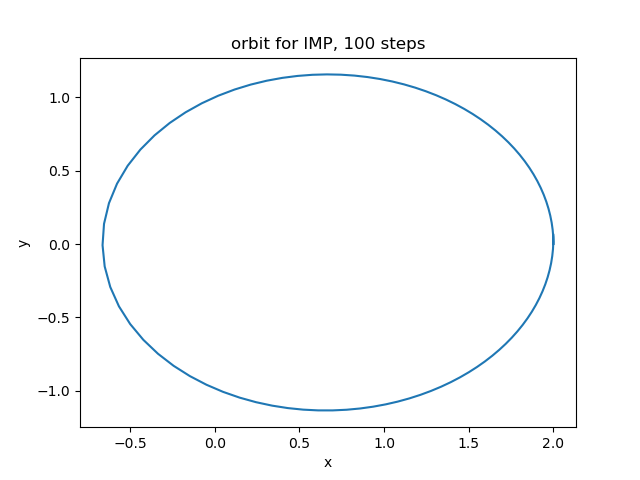
\includegraphics[scale=.3]{hw5 IMP orbit 100 steps}
	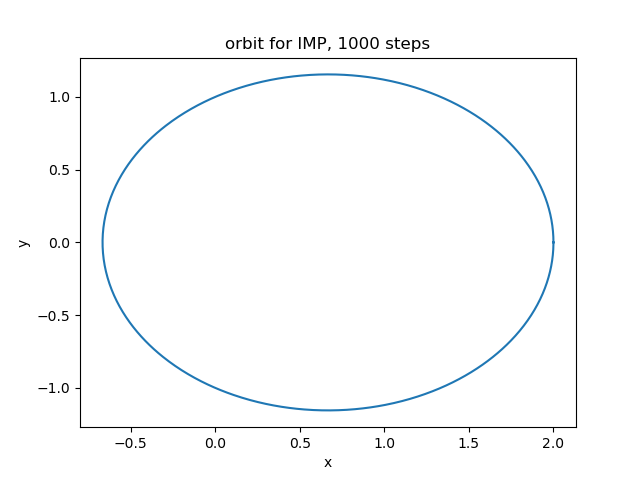
\includegraphics[scale=.3]{hw5 IMP orbit 1000 steps}
	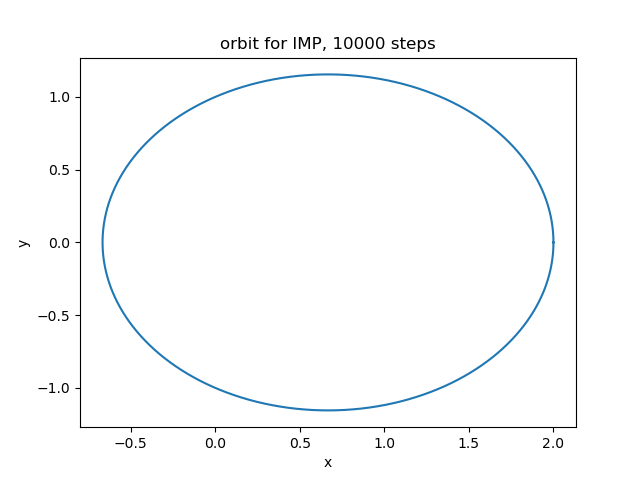
\includegraphics[scale=.3]{hw5 IMP orbit 10000 steps}
	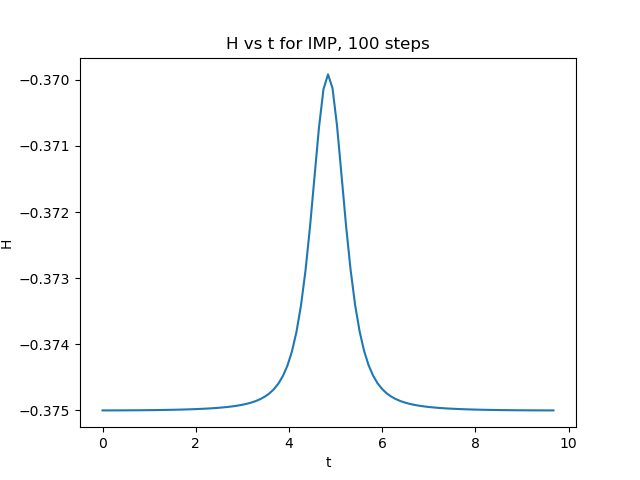
\includegraphics[scale=.3]{hw5 IMP ham 100 steps}
	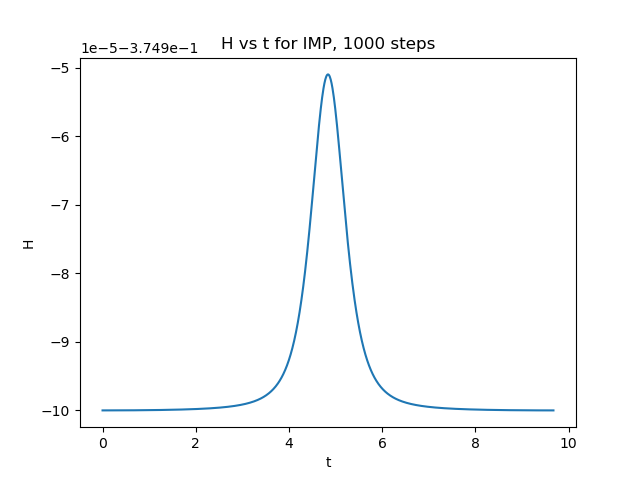
\includegraphics[scale=.3]{hw5 IMP ham 1000 steps}
	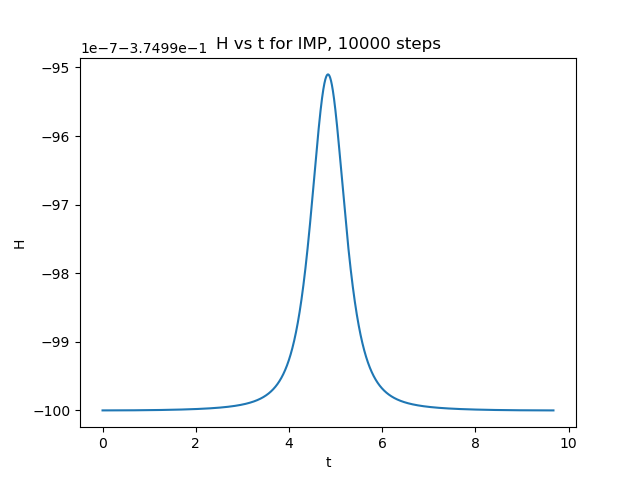
\includegraphics[scale=.3]{hw5 IMP ham 10000 steps}
\end{center}


\item In the Stoermer--Verlet method (SV), set $p:=(u,v)$ and $q:=(x,y)$. The Hamiltonian is
$$H(p,q) = T(p) + U(q),
\quad T(p) := \frac12u^2 + \frac12v^2,
\quad U(q) := -(x^2 + y^2)^{-1/2}$$
so that
$$\ptl_pH(p,q) = \grad T(p) = \m{u \\ v},
\quad \ptl_qH(p,q) = \grad U(q) = \m{x(x^2+y^2)^{-3/2} \\ y(x^2+y^2)^{-3/2}}$$
In the method derived in problem 1, replace $T'$ and $U'$ by $\grad T$ and $\grad U$.
$$q_{n+1} = q_n + h\grad T\br{p_n - \frac12hU'(q_n)}$$
$$p_{n+1} = p_n - \frac12h\sbr{U'(q_n) + \grad U\br{q_n + h\grad T\br{p_n - \frac12h\grad U(q_n)}}}$$
Below are the same plots as in part (b) but using SV instead.

\begin{center}
	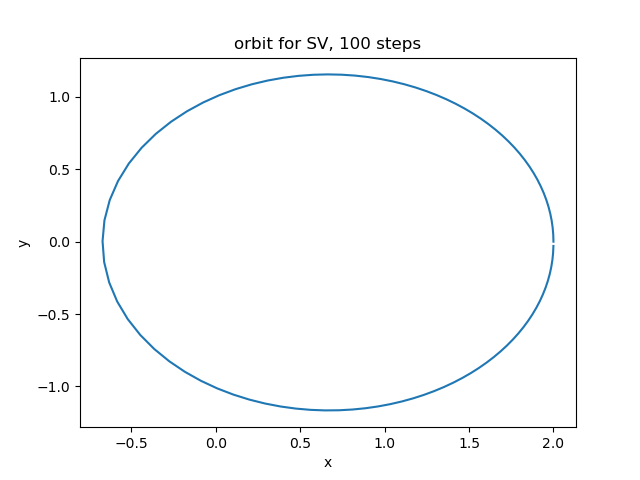
\includegraphics[scale=.3]{hw5 SV orbit 100 steps}
	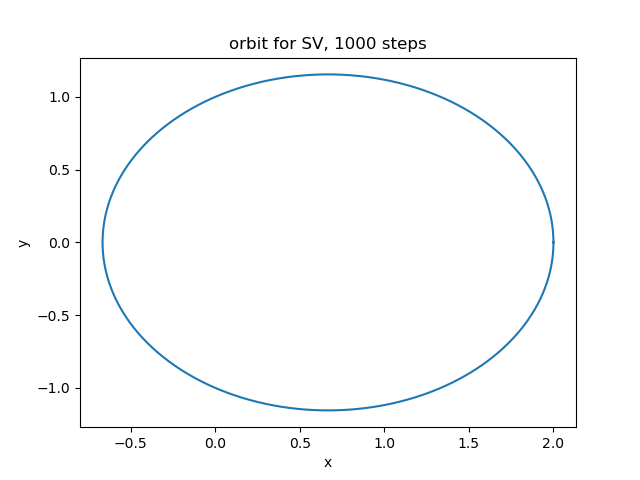
\includegraphics[scale=.3]{hw5 SV orbit 1000 steps}
	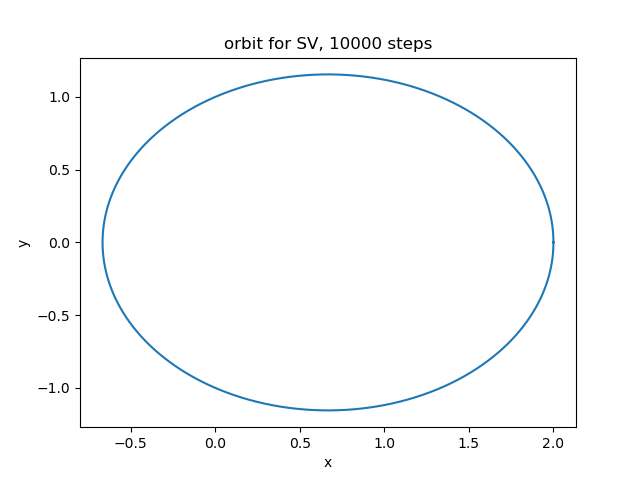
\includegraphics[scale=.3]{hw5 SV orbit 10000 steps}
	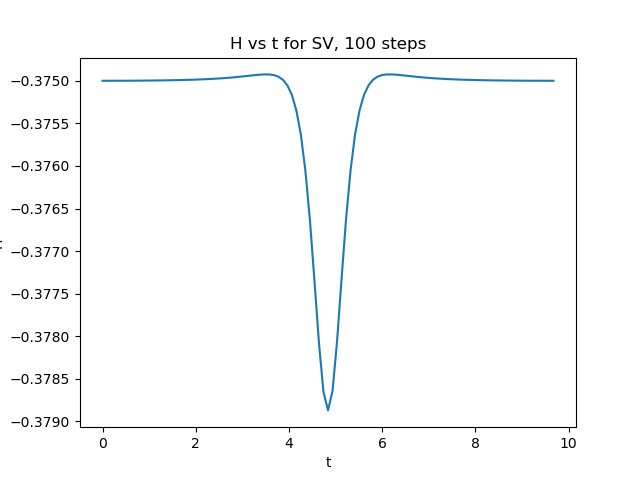
\includegraphics[scale=.3]{hw5 SV ham 100 steps}
	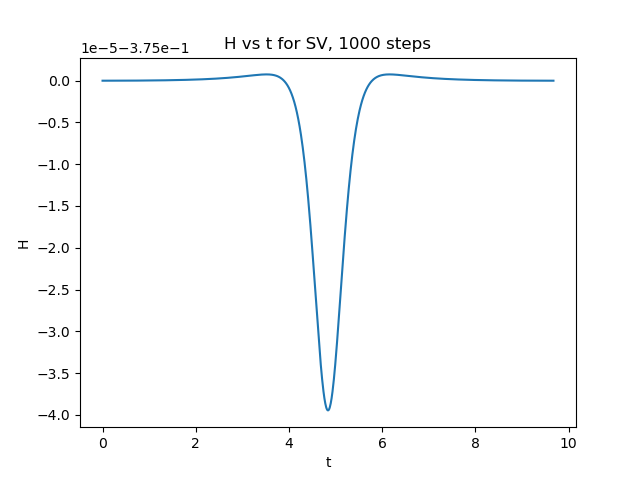
\includegraphics[scale=.3]{hw5 SV ham 1000 steps}
	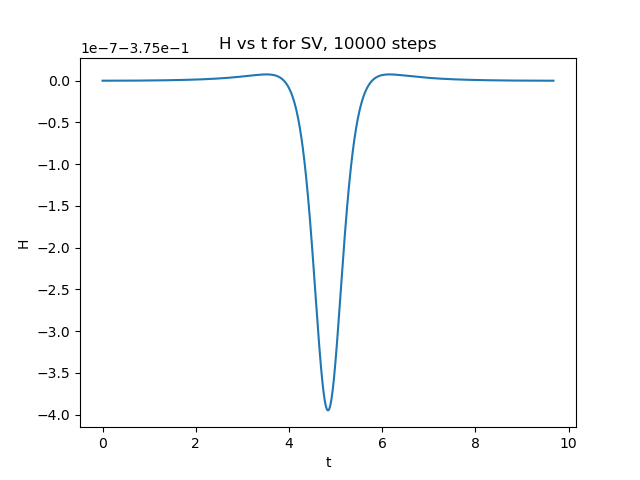
\includegraphics[scale=.3]{hw5 SV ham 10000 steps}
\end{center}


\item To compare accuracy, we compare the differences in the maximum and minimum Hamiltonian, listed in the order corresponding to the number of steps taken per period: 100, 1000, 10000. The differences for IMP are:
$$0.005081464348190012,
\quad 4.900006001706814\cdot10^{-5},
\quad 4.898265737462992\cdot10^{-7}$$
The differences for SV are:
$$0.0039456711144399415,
\quad 4.022530826314208\cdot10^{-5},
\quad 4.0233147502455324\cdot10^{-7}$$
The differences for SV are smaller than those for IMP, so SV is more accurate than IMP.

\end{enumerate}
\sep



\tbf{Problem 3.} Using $f(z)=\lambda z$,
$$k = f\br{z_n + \frac12hk}
= \lambda\br{z_n + \frac12hk}
= \lambda z_n + \frac12h\lambda k
\imp \br{1 - \frac12h\lambda}k = \lambda z_n
\imp k = \lambda\br{1 - \frac12h\lambda}\inv z_n$$
$$\imp z_{n+1} = z_n + hk
= z_n + h\lambda\br{1 - \frac12h\lambda}\inv z_n
= \sbr{1 + h\lambda\br{1 - \frac12h\lambda}\inv}z_n$$
Set $w:=h\lambda$, so
$$1 + h\lambda\br{1 - \frac12h\lambda}\inv = 1 + w\br{1 - \frac12w}\inv
= 1 + w\br{\frac{2-w}{2}}\inv
= 1 + \frac{2w}{2-w}
= \frac{2-w+2w}{2-w}
= \frac{w+2}{2-w}$$
$$\imp z_{n+1} = \frac{w+2}{2-w}z_n \imp z_n = \br{\frac{w+2}{2-w}}^nz_0$$
Now $w=x+iy$ where $x:=\Re w$ and $y:=\Im w$. Then
$$z_n \app[n][\infty] 0
\iff \abs{\frac{w+2}{w-2}}<1
\iff |w+2| < |w-2|
\iff |w+2|^2 < |w-2|^2
\iff (x+2)^2 + y^2 < (x-2)^2 + y^2$$
$$\iff (x+2)^2 < (x-2)^2
\iff x^2 + 4 + 4x < x^2 + 4 - 4x
\iff 4x < -4x
\iff 8x < 0
\iff x < 0$$
Thus the RAS is $\brc{w\in\bC: \Re w<0}$.
	
\end{document}